\part{Multi-tenant Cloud Application}

\begin{frame}{What is a Multi-tenant Cloud Application?}
\textit{One application instance can serve requests from multiple customers.}
\vfill
\begin{block}{Definition}
\textbf{Multi-tenancy} refers to a software architecture in which multiple customers (a.k.a. tenants) share the 
same technical resources while keeping \textbf{I}dentity and \textbf{A}ccess \textbf{M}anagement (IAM) and data separated.
\end{block}
\vfill
\begin{figure}
        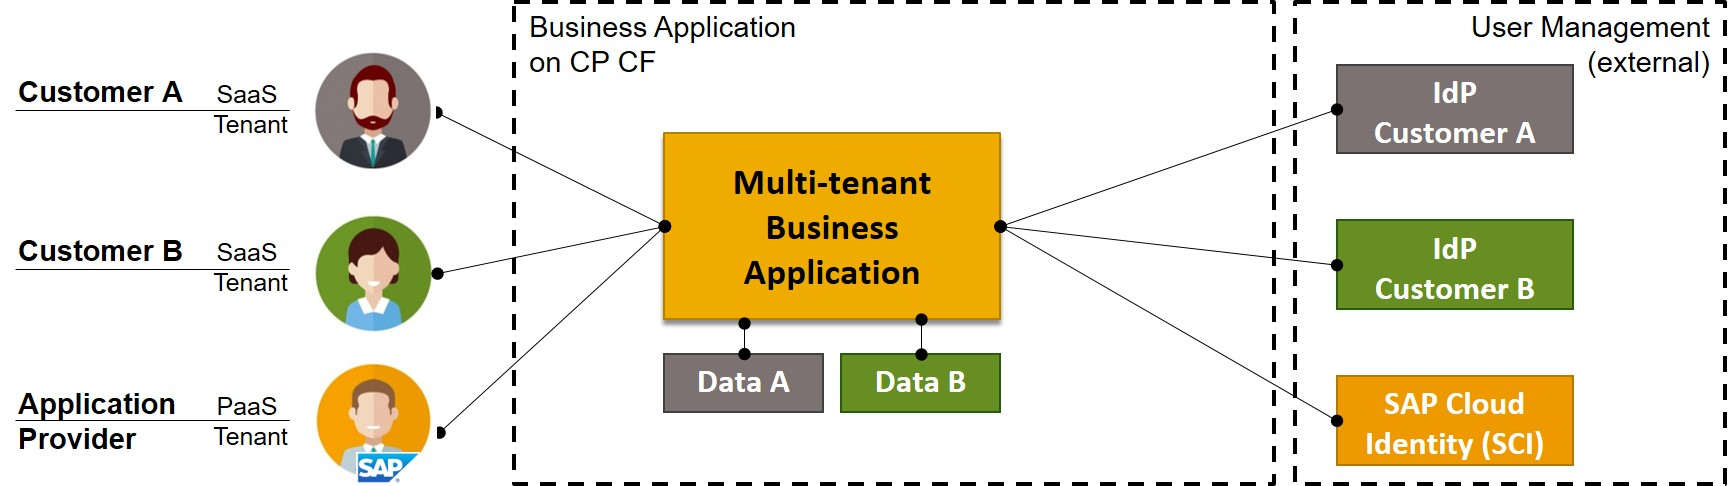
\includegraphics[width=0.9\textwidth]{../MultiTenancy/images/MultiTenantApplication_Simple}
\end{figure}
%\textbf{Questions addressed}
%\begin{itemize}
%	\item What is the Tenant Concept on SAP CP CF?
%	\item How to setup a Tenant aware Identity \& Access Management? 
%	\item Data Isolation - which aspects and degrees to consider?
%	\item How to separate DB Schema using HANA Instance Manager?
%\end{itemize}
\end{frame}

\begin{frame}[t]{Multi-tenancy @SAP CP}
\small
\begin{enumerate}[<+->]
\item In SAP CP, each tenant has a separate \textbf{Identity Zone in SAP UAA}.
\\This allows isolated User Management per tenant. 
\item This concept includes a multi-tenant enabled AppRouter which is deployed with a multi-tenant application. 
A multi-tenant application is called with a \textbf{tenant-specific URL}. URL schema: 
\colorlink{https://<tenant>.<app>.<domain>}{https://<tenant>.<app>.<domain>}
\item SAP CP provides \textbf{onboarding services} to create new tenants
\\and to \textbf{subscribe} to a multi-tenant application. 
\item A multi-tenant application can implement a \textbf{callback method} 
\\to be notified on new subscriptions.
\item An \textbf{Instance Manager}, which manages service instances transparently to applications, is provided; thus it can be used for managing tenant specific HANA service instances.
\end{enumerate}
\end{frame}

\begin{frame}[t]{Identity Zones separate User Management}{\ldots into different Security Realms for XSUAA}
\small
\begin{enumerate}
\item In SAP CP CF, each tenant has a separate \textbf{Identity Zone in SAP UAA}.
\\This allows isolated User Management per tenant. 
\end{enumerate}
\vfill
\only<1>{
    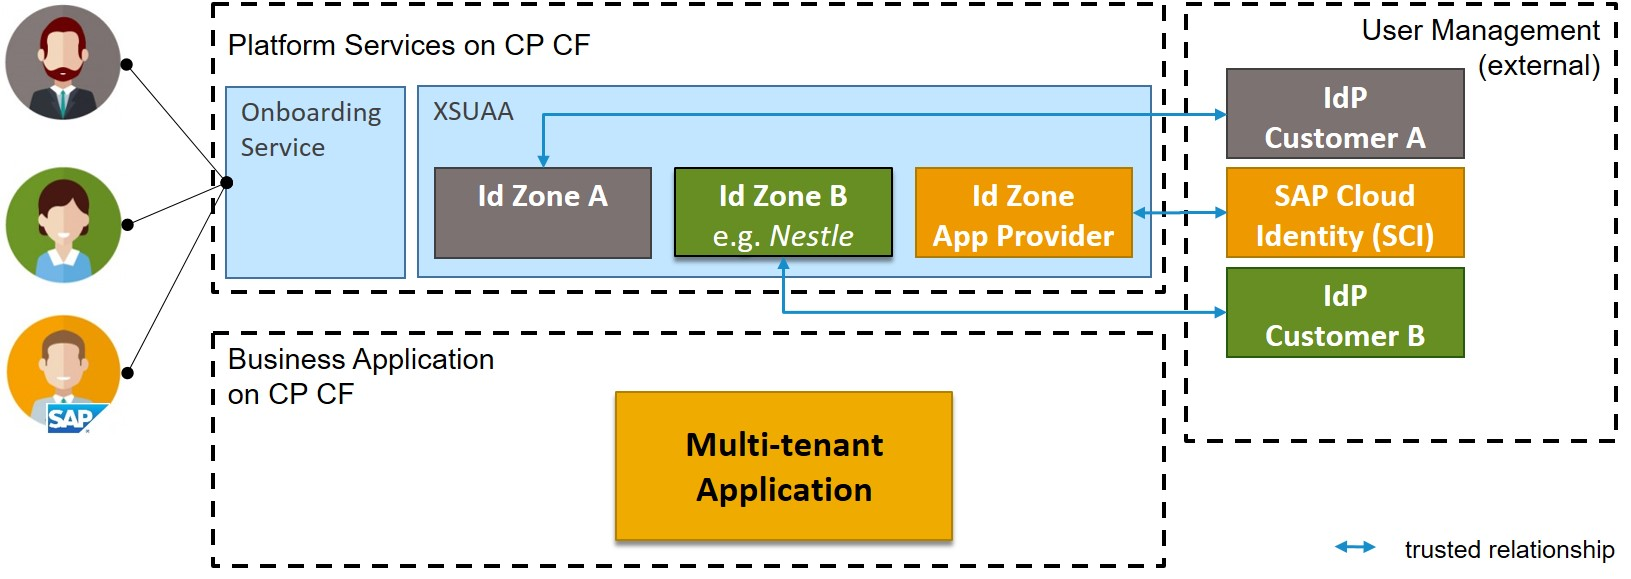
\includegraphics[width=\textwidth]{../MultiTenancy/images/IdentityZones}
}
\only<2>{
    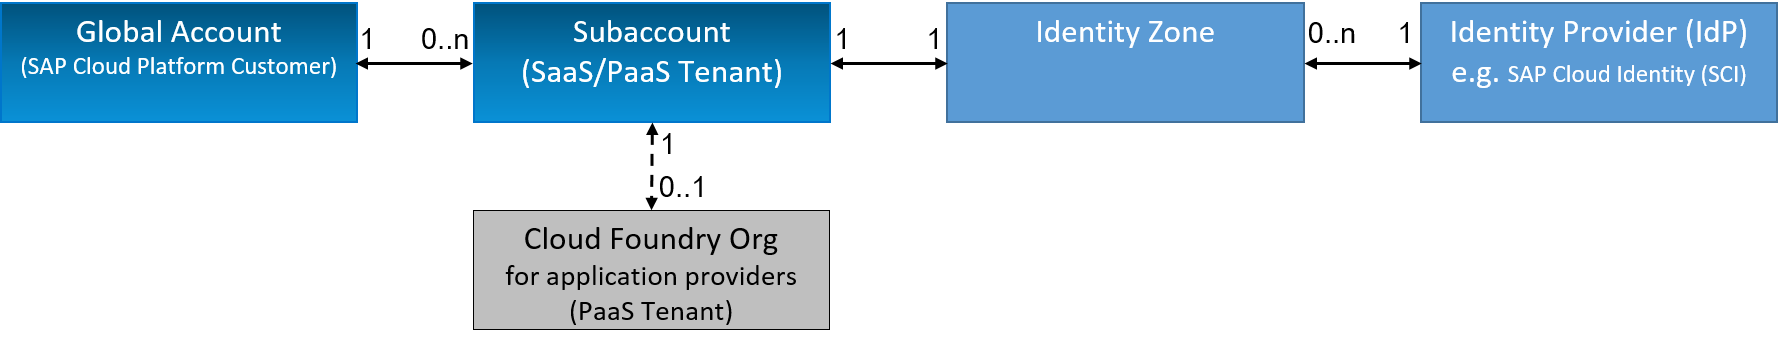
\includegraphics[width=\textwidth]{../MultiTenancy/images/Tenant-IdZone-IdP}
    \vfill
    Each customer (SaaS tenant) and application provider (PaaS tenant) requires a \textbf{Subaccount} to attach his \textbf{IdP}s via his corresponding \textbf{Identity Zone}.
}
\only<3>{
    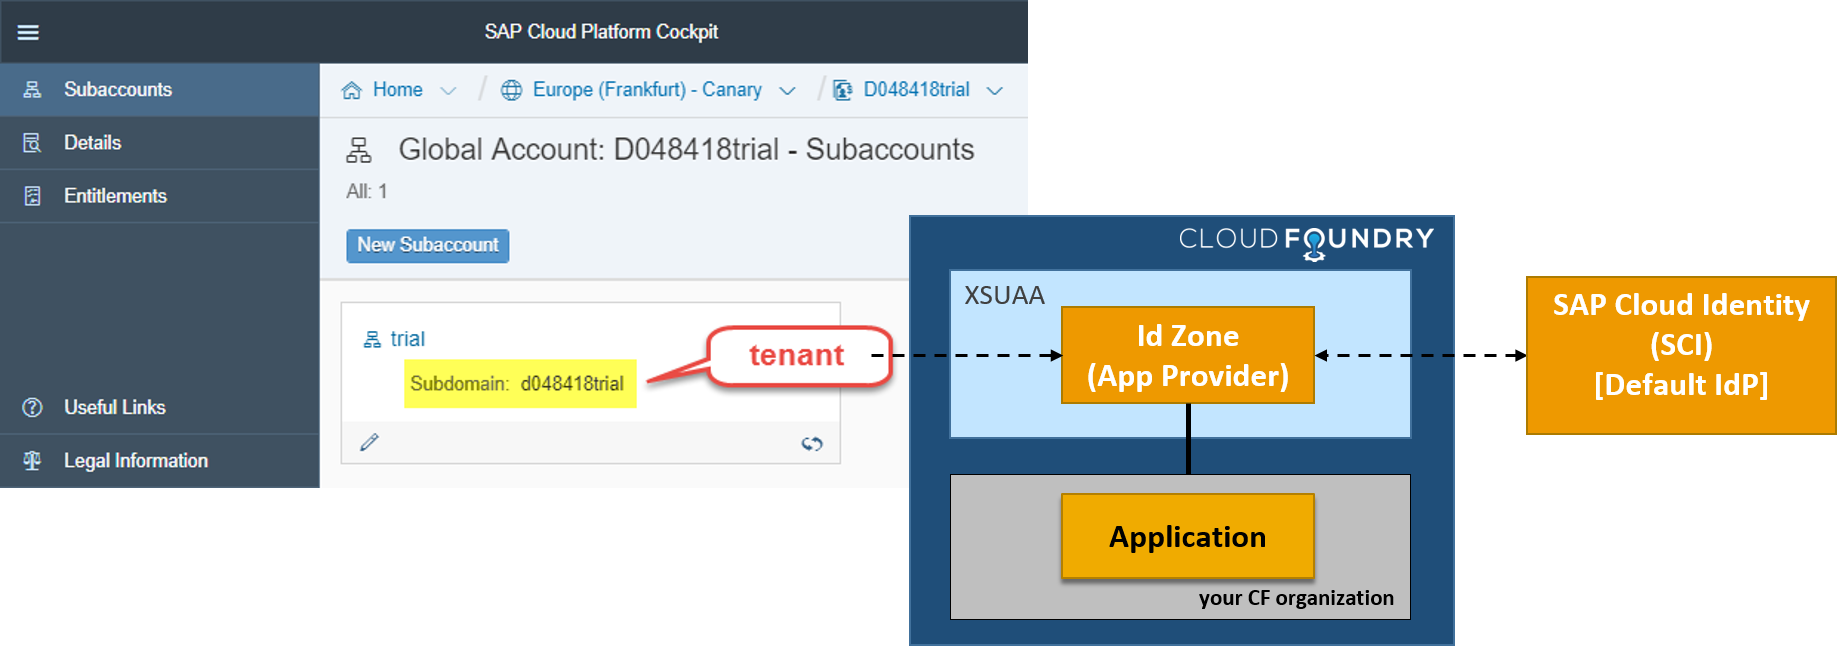
\includegraphics[width=\textwidth]{../MultiTenancy/images/SubAccountSubDomainTenant}
    \vfill
    During onboarding the \textbf{Identity Zone} e.g. \textit{d012345trial} is created automatically. 
    \\The \textbf{Subdomain} represents the \textbf{Tenant} used in the Cloud Foundry environment.
    %In the PaaS Use Case, the Id-Zone of the Subaccount is assigned to the CF Org of the Subaccount 
}
\only<4>{
    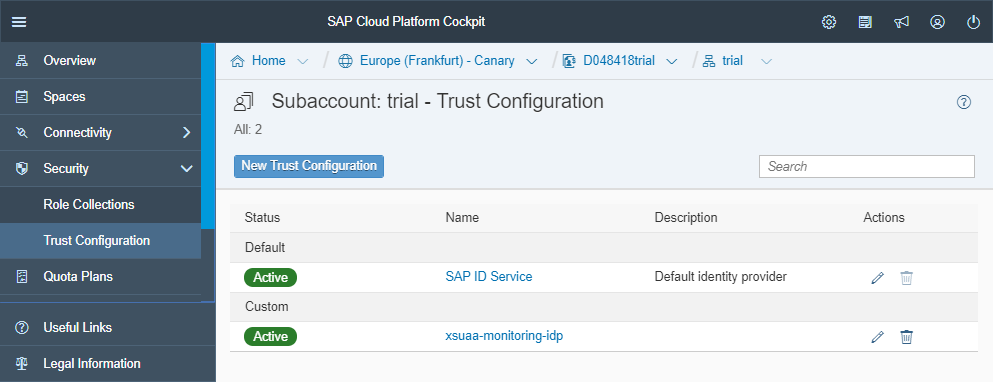
\includegraphics[width=0.9\textwidth]{../MultiTenancy/images/ConfigureTrustToIdP}
    \vfill
    Per Subaccount the administrator on customers side needs to establish trust between XSUAA Identity Zone and customer IdP.
}
\end{frame}


\begin{frame}[t]{Tenant-Aware Application Security Setup}
\small
\begin{enumerate}
\setcounter{enumi}{1}
\item This concept includes a multi-tenant enabled AppRouter which is deployed with a multi-tenant application. 
A multi-tenant application is called with a \textbf{tenant-specific URL}. URL schema: 
\colorlink{https://<tenant>.<app>.<domain>}{https://<tenant>.<app>.<domain>}
\end{enumerate}
\vfill
\only<1>{
    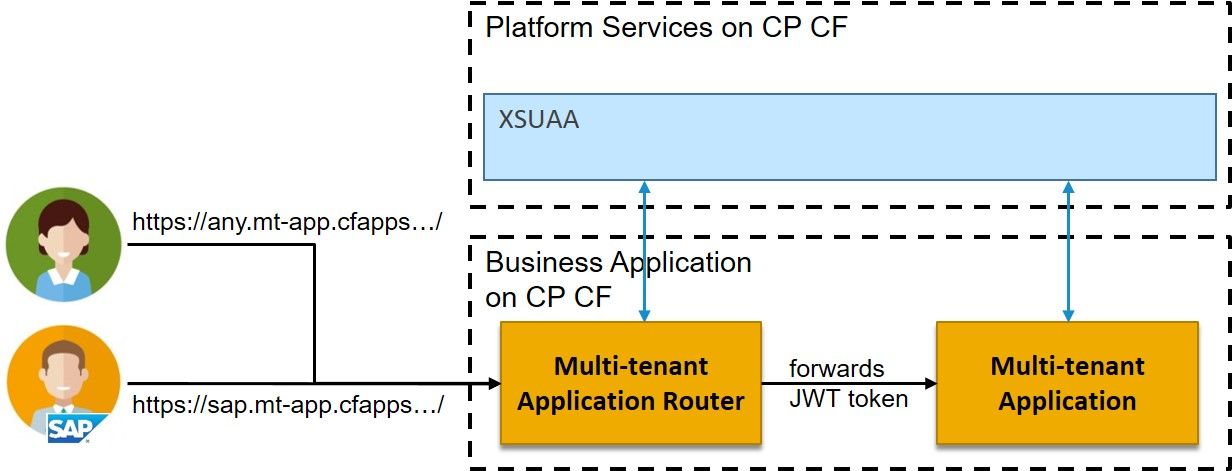
\includegraphics[width=0.8\textwidth]{../MultiTenancy/images/TenantAwareApplciationSetup}
    \vfill
    \colorlink{https://github.wdf.sap.corp/cc-java-dev/cc-coursematerial/blob/master/Security/Exercise_22_DeployApplicationRouter.md}{Related Exercises: 22 - 24}
	\footnotesize
	\\Note: in the canary landscape the URL schema is \colorlink{https://<tenant>-<app>.<domain>}{https://<tenant>-<app>.<domain>}
	\scriptsize
	\\(requires no SSL certificate configuration)
}
\only<2>{
    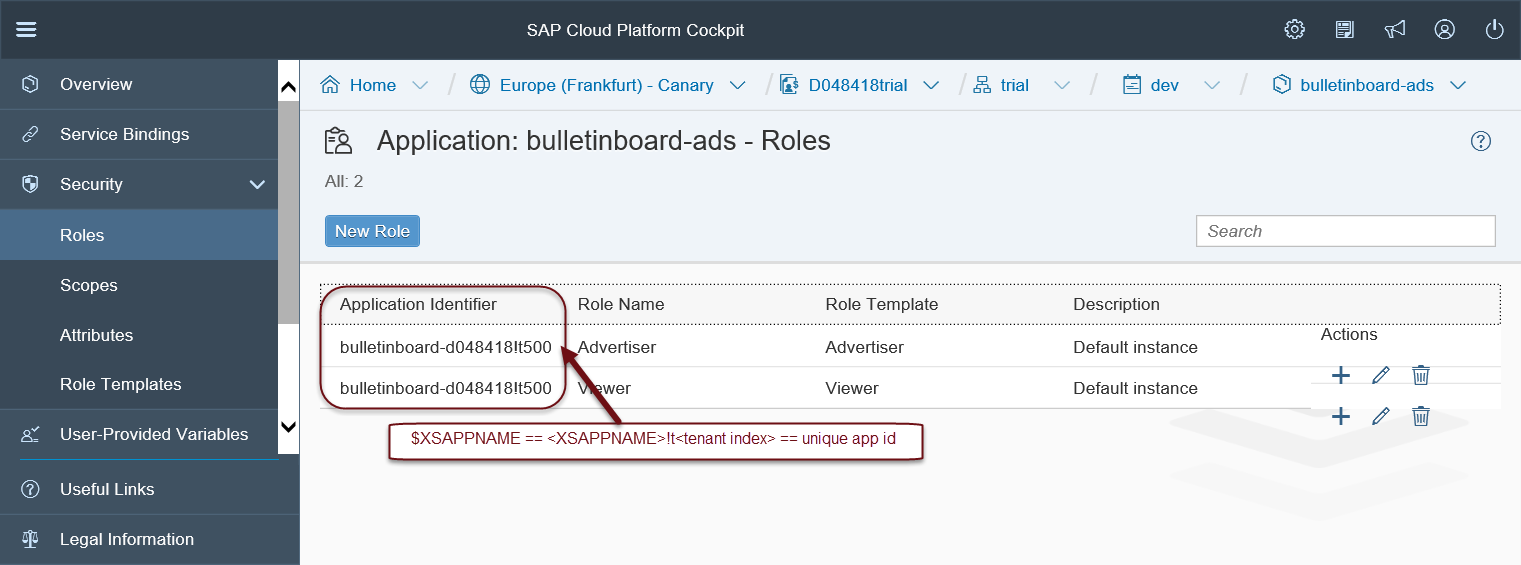
\includegraphics[width=0.9\textwidth]{../MultiTenancy/images/XSAPPNAME_TenantIndex_explained}
    \vfill
    \scriptsize
    Note: XSUAA creates tenant index to ensure unique appids, when the same application is deployed into several spaces of the CF organization. XSAPPNAME is suffixed with \codealt{t!<tenant index>}.
}  
\end{frame}


\begin{frame}[t]{Application Subscription}
\small
\begin{enumerate}
\setcounter{enumi}{2}
\item SAP CP provides \textbf{onboarding services} to create new tenants 
\\and to \textbf{subscribe} to a multi-tenant application. 
\end{enumerate}
\vfill
\only<1>{
    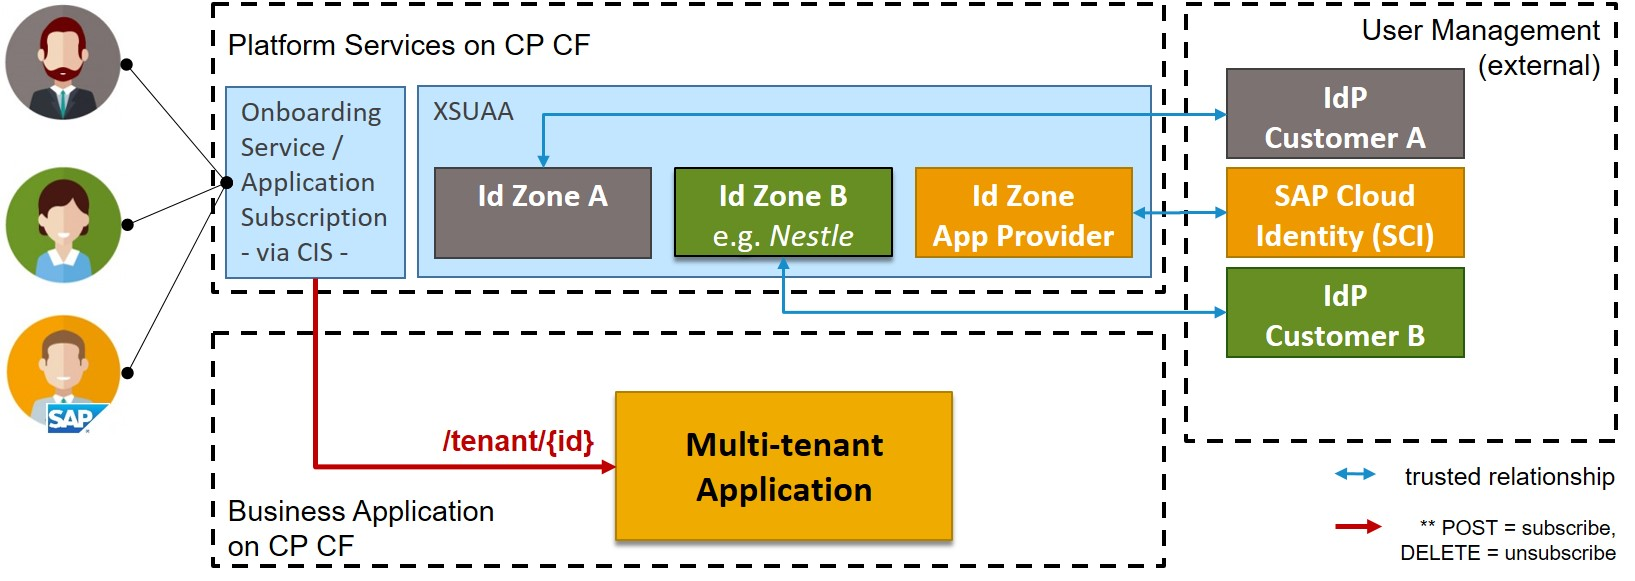
\includegraphics[width=0.9\textwidth]{../MultiTenancy/images/ApplicationSubscription}
    \scriptsize
    \newline
    \vfill
    During subscription the application and its authorization-model (\codealt{xs-security.json}) are exposed in the Identity Zone of the respective Subaccount.
    Subscription callbacks of applications are called.
}

\only<2>{
    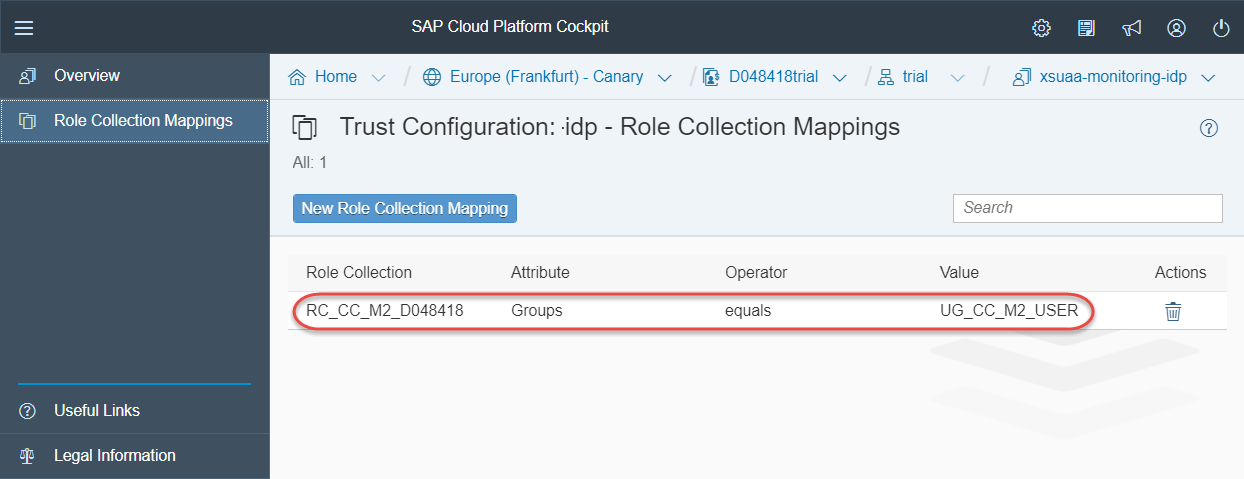
\includegraphics[width=0.9\textwidth]{../MultiTenancy/images/AdministrateSubaccounts}
    \vfill
    Now you can create \textbf{Roles}, \textbf{RoleCollections} and assign them to \textbf{SAML2 User Groups} or directly to User Ids (e.g. email).
}
\end{frame}



%----------
\begin{frame}[t,fragile]{Callbacks for Tenant On-/Offboarding}
\small
\begin{enumerate}
\setcounter{enumi}{3}
\item A multi-tenant application can implement a \textbf{callback method} 
\\to be notified on new subscriptions
    \begin{itemize}
    \item to prepare db schema, create tenant-specific data/config, …
    \end{itemize}
And \textbf{another callback} to provide dependent applications.
\end{enumerate}
\vfill
You need to bind your application to a \codealt{Local Provisioning Service} instance. 
\vfill
SAP-internal documentation on \colorlink{https://uacp2.hana.ondemand.com/doc/DRAFT/53ddfc1f9f88403b82d6f975e84e12a3/T11a\%202016/en-US/frameset.htm?9a80c26d9b614279bc97d07061a28f9b.html}{SAP CP Help}
\end{frame}


\begin{frame}[fragile]{Make your Application Tenant-aware - Part 1}
\textbf{How to fetch tenant from the JWT token ("zid")}
\\\begin{lstlisting}[language=Java]
String tenant = SecurityContext.getUserInfo().getIdentityZone();
\end{lstlisting}
\vfill
\textbf{Initialize Log Context with tenant}
\\\begin{lstlisting}[language=Java]
import static com.sap.hcp.cf.logging.common.customfields.CustomField.customField;
...
logger.info("Log tenant info with custom field {}", customField("tenant", tenantValue"));
\end{lstlisting}
\vfill
\textbf{Apply tenant to the downstream service routes}
\\\begin{lstlisting}[language=Java]
String uriTemplate = "https://{tenant}-approuter.mydomain/ads/api/v1/ads/";
URI url = new UriTemplate(uriTemplate).expand(tenant);
HttpEntity<String> request = new HttpEntity<>("My Content");
ResponseEntity<String> response = restTemplate.exchange(url, HttpMethod.GET, request, String.class);
\end{lstlisting}
\end{frame}


\begin{frame}[t,fragile]{Make your Application Tenant-aware - Part 2}{Excursion - Setup Tenant Context for each Request}
\begin{block}{Example \codealt{TenantContext}:}
\begin{lstlisting}[language=Java,belowskip=-3mm,aboveskip=0mm]
public class TenantContext {
    final public static String DEFAULT_TENANT = "public"; 
    //gives each thread its own local variable
    private static ThreadLocal<String> currentTenant = new ThreadLocal<String>() { 
        @Override protected String initialValue() {
            return DEFAULT_TENANT;//required for initial startup
    }};
    public static void setCurrentTenant(String tenantId) {
        currentTenant.set(tenantId);
    }
    public static String getCurrentTenant() {
        return currentTenant.get();//provides a dedicated instance 
    }
    public static void clear() {
        currentTenant.remove();//avoid memory leaks:release it for garbage coll.
    }
}
\end{lstlisting}
\end{block}
\scriptsize
For each request initialize \codealt{TenantContext} as part of a \codealt{HandlerInterceptor} (\colorlink{https://github.wdf.sap.corp/LCA-POCs/lca-core/blob/master/src/main/java/com/sap/cloud/lca/core/multitenancy/TenantInterceptor.java}{Example})
\end{frame}



%----------Data Isolation
\begin{frame}[t,fragile]{Data Isolation}
\small
One common question raised while dealing with SaaS architecture is:\\"Should there be an isolated database for every single customer or should multiple customers share a database?"
\vfill
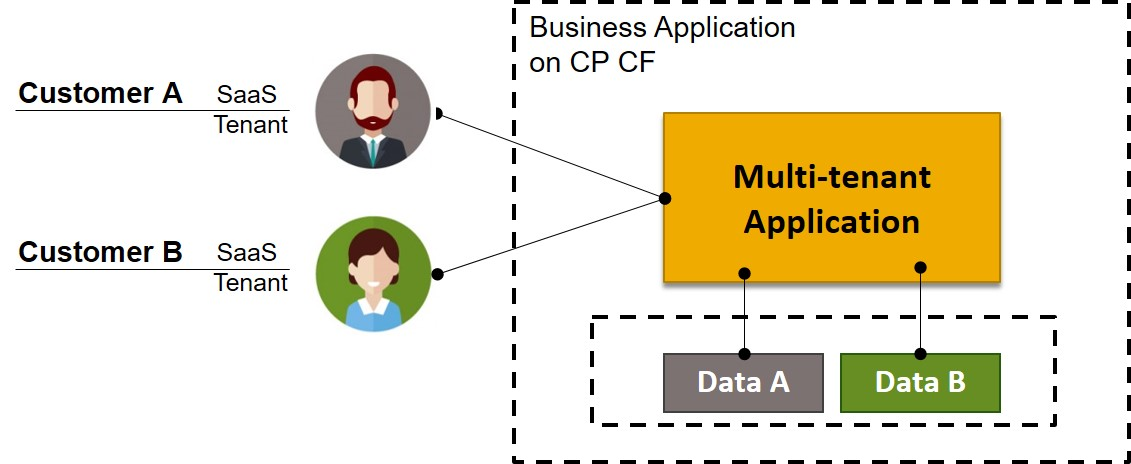
\includegraphics[width=0.9\textwidth]{../MultiTenancy/images/DataIsolation}
\end{frame}

\begin{frame}[t,fragile]{Data Isolation - Aspects and Degrees}
\small
Degrees of (data) isolation (\colorlink{https://wiki.wdf.sap.corp/wiki/display/PSSEC/SEC-253}{PS-SEC 253})
\vfill
\begin{itemize}
\item \textbf{Shared schema:} individual tables contain \textbf{tenant discriminator column}
\\(e.g. MANDT) 
\item \textbf{Separate schemas:} Each tenant has its own \textbf{database schema (or HDI container)} but shares a DB (recommended approach)
\item \textbf{Separate databases (premium approach):} Each tenant has its own dedicated database (by process / physical) to provide “bad neighborhood protection” in terms of data and failure isolation, resource consumption, performance (cache, I/O, …) etc. In HANA this would be a separate Multitenant Database Container (logical database) per customer.
\end{itemize}
\vfill
\textbf{Aspects to be considered}
Customer requirements for: data security/isolation, performance guarantees, extensibility, reliability, disaster recovery (backup and restore),\ldots
\end{frame}


\begin{frame}[t,fragile]{Tenant Discriminator Column}

\begin{block}{Example using EclipseLink}
\begin{lstlisting}[language=Java,belowskip=0mm,aboveskip=0mm]
import static org.eclipse.persistence.annotations.MultitenantType.*;

@Entity
@Table(name = "advertisements")
@Multitenant(SINGLE_TABLE) 
@TenantDiscriminatorColumns({ 
    @TenantDiscriminatorColumn(name = "TENANT_ID"),
    @TenantDiscriminatorColumn(name = "TENANT_CODE")})
public class Advertisement {
}
\end{lstlisting}
\end{block}
\vfill
\textbf{References}
\begin{itemize}
\item \colorlink{http://wiki.eclipse.org/EclipseLink/UserGuide/JPA/Advanced_JPA_Development/Single-Table_Multi-Tenancy}{Multi-tenancy annotations in JPA (EclipseLink 2.3)}
\item \colorlink{https://help.hana.ondemand.com/help/frameset.htm?54a76156cd114e5d928642b8dde47b91.html}{Multi-tenant Applications” in SAP CP classic Documentation}
\end{itemize}
\end{frame}


\begin{frame}[t,fragile]{Tenant Discriminator Schema}
Hibernate natively supports Schema-based multi-tenancy e.g. in conjunction with PostgreSQL. It requires three main components:
\begin{itemize}
\item \textbf{Configuration}\\Wiring up Hibernate correctly
\item \textbf{CurrentTenantIdentifierResolver}\footnote{Depends on \codealt{TenantContext} class that was introduced previously.}\\Class responsible for resolving the correct tenant, map tenant to db schema. 
\item \textbf{MultiTenantConnectionProvider}\\Class responsible for providing and closing tenant connections.
\end{itemize}
\vfill
\textbf{References}
\begin{itemize}
\item \colorlink{http://stuartingram.com/2016/10/02/spring-boot-schema-based-multi-tenancy/}{SpringBoot Tutorial}
\item \colorlink{https://github.wdf.sap.corp/LCA-POCs/lca-core/}{Example on SAP GitHub: Legal Content Assembly (PoC)}
\end{itemize}
\end{frame}

\begin{frame}[t]{HANA Multitenant DB Container (MDC)}{Using HANA Instance Manager}
\small
\begin{enumerate}
\setcounter{enumi}{4}
\item Bind to \textbf{HANA instance manager (managed\_hana)} that manages tenant specific HANA service instances transparently to the application.

\end{enumerate}
\vfill
\only<1>{
    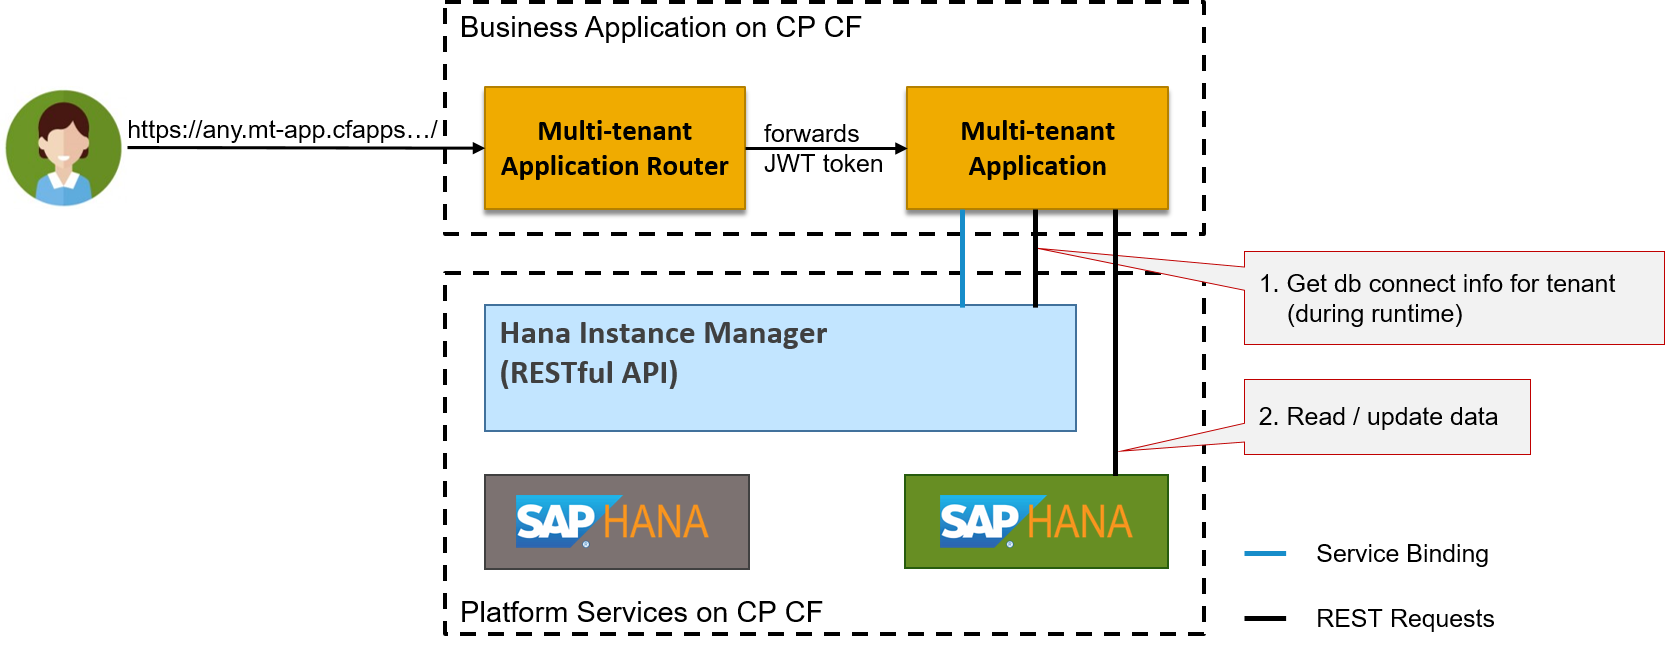
\includegraphics[width=0.9\textwidth]{../MultiTenancy/images/TenantSpecificDBSchemaUsingHANAInstanceManager}
    \vfill
    \textbf{Recommendations}: cache credentials and connection info to hana service instance and pool open connections
}
\end{frame}



\begin{frame}{References}
\small
\begin{itemize}
\item \colorlink{https://wiki.wdf.sap.corp/wiki/display/IoTArch/Multitenancy}{Wiki: Multitenancy for SAP CP CF - Concept Paper.pdf}
\item \colorlink{https://wiki.wdf.sap.corp/wiki/display/xs2/Multi-Tenancy}{XSA Wiki: Multi Tenancy}
\item \colorlink{https://uacp2.hana.ondemand.com/doc/DRAFT/53ddfc1f9f88403b82d6f975e84e12a3/T11a\%202016/en-US/frameset.htm?fe9b5fb6cf194413b703a7062498911b.html}{SAP-internal Documentation}
\item \colorlink{https://jam4.sapjam.com/groups/ApFhQ0NCGAzAtXQWsdqB3B/overview_page/p8JIXj2pstIcY7TegLyOp8}{Cloud Foundry JAM: How to Onboard as Application Provider}
\item \colorlink{https://jam4.sapjam.com/groups/DRuoC97ApSanbbXx20g4kb/overview_page/DbkVBP2VFuhYrVqiCoRRmQ}{SAP CP Security JAM: Getting Started}
\item \colorlink{https://wiki.wdf.sap.corp/wiki/display/xs2/Application+Managed+Service+Instances}{XSA Wiki: Application Managed Service Instances - Concept Paper}
\item \colorlink{https://jam4.sapjam.com/groups/ZBxGNs1cJ5Z7OVkQRwBM0G/overview_page/CAOFv7dO1fHvikIDIRfj6v}{One CP JAM: Find here Cockpit Presentations etc.}
\end{itemize}
\vfill
\textbf{References related to HANA Instance Manager}
\begin{itemize}
    \item \colorlink{https://wiki.wdf.sap.corp/wiki/pages/viewpage.action?pageId=1884767923}{XSA Instance Manager Client Library - for Java}
    \item \colorlink{https://github.wdf.sap.corp/IndustryCloudFoundation/multi-tenant-library}{ICD Multi-tenant Library - for Java}
\end{itemize}
\end{frame}

